\documentclass[a4paper]{article}

\usepackage[english]{babel}
\usepackage[utf8]{inputenc}
\usepackage{amsmath}
\usepackage{graphicx}
\usepackage{hyperref}

\title{AST4320 - Assignment 3}

\author{Metin San}

\date{\today}

\begin{document}
\maketitle

\section*{Exercise 1}
\subsection*{a)}
We assume that the intergalactic medium (IGM) contains only hydrogen and helium with
respective mass fractions $X = 0.76$ and $Y = 0.24$ respectively. In general, the mean
molecular weight $\mu$ is given as 

\begin{equation}\label{eq:mu}
    \mu = \sum_i \left ( \frac{X_i}{A_i} \right )^{-1},
\end{equation}

\noindent where $X_i$ are the atomic species of consideration, which in our case is $X$ and
$Y$ for hydrogen and helium, and $A_i$ is the atomic weight of the species divided by the
ionization number. We will assume that the entire IGM is completely ionized so that $A_X =
1/2$ because the atomic weight of hydrogen is 1 and the ionization number is 2 as one electron
and 1 proton is produced. Similarly, $A_Y = 4/3$ as the atomic weight of helium is 4, and 3
particles are produced (1 helium core and 2 electrons). Using these numbers we can calculate
the mean molecular weight of the IGM

\begin{equation}\label{eq:muIGM}
    \mu = \frac{1}{2X + (3/4)Y} = 0.5882.
\end{equation}

\subsection*{b)}
The Jeans mass is given as 

\begin{equation}\label{eq:jean}
    M_J = \frac{\pi}{6} \rho \lambda_J^3,
\end{equation}

\noindent where $\rho$ is the density and $\lambda_J$ is the Jeans length given as

\begin{equation}\label{eq:jeanlen}
    \lambda_J = c_s \left(\frac{\pi}{G \rho} \right)^{1/2}.
\end{equation}

\noindent Here, $c_s$ is the speed of sound given as

\begin{equation}\label{eq:sound}
    c_s = \left( \frac{k_B T}{\mu m_p} \right)^{1/2}.
\end{equation}

\noindent Since we are considering the IGM, the density is given as

\begin{equation}\label{eq:rho}
    \rho = \rho_m(1+z)^3 = \Omega_m \rho_c (1+z)^3,
\end{equation}

\noindent where we have used that $\Omega_m = \rho_m / \rho_c = 0.308$ where $\rho_c \approx 10^{-26}$kg m$^{-3}$ is the critical density. If we now use the definitions in equations \eqref{eq:sound}, \eqref{eq:rho}, we can rewrite the expressions of the Jeans length and mass in terms of redshift. The Jeans mass is then given as

\begin{equation}\label{eq:jeanfinal}
    M_J = \frac{\pi^{5/2}}{6} \left( \frac{k_B T}{G \mu m_p} \right)^{3/2} (\Omega_m \rho_c)^{1/2} (1+z)^{3/2},
\end{equation}

\noindent and similarely the Jeans length is given as

\begin{equation}\label{eq:jeanlenfinal}
    \lambda_J = \left( \frac{\pi k_B T}{G \mu m_p \Omega_m \rho_c} \right)^{1/2} (1+z)^{-3/2}.
\end{equation}

\noindent If we use that the IGM has a temperature of $T = 10^4$K, then the Jeans Mass at a redshift $z = 4$ with the corresponding wave number $k$ is equal to 

\begin{equation}\label{eq:jeans z=4}
    M_J(z=4) = 5.515 \times 10^{15}\mathrm{kg}, \qquad k = \frac{2\pi}{\lambda_J(z = 4)} = 1.516 \times 10^{-21}\mathrm{m}^{-1}.
\end{equation}


\section*{Exercise 2}
In the lectures we derived that the total optical depth of the ionized IGM due to
electron scattering is given by

\begin{equation}\label{eq:tau}
    \tau _ { \mathrm { e } } ( z ) = c \int _ { 0 } ^ { z } \frac { n _ { e } ( z )
    \sigma _ { \mathrm { T } } d z } { ( 1 + z ) H ( z ) },
\end{equation}

\noindent where $\sigma _ { \mathrm { T } } = 6.65 \times 10^{-25}$ is the cross-section
for electron scattering, $\overline { n } _ { \mathrm { H } } ( z ) \sim 1.9 \times 10 ^
{ - 7 } ( 1 + z ) ^ { 3 } \mathrm{cm}^{-3}$ is the average number density of hydrogen.
We have the following cosmological parameters $\Omega _ { \Lambda } = 0.692 , 
\Omega _ { m } = 0.308 \text { and } \Omega _ { r } = 0$. $H(z)$ is the Hubble parameter
and is given as

\begin{equation}\label{eq:hub}
    H ^ { 2 } ( z ) = H _ { 0 } ^ { 2 } \left( \Omega _ { m } ( 1 + z ) ^ { 3 } + \Omega
    _ { r } ( 1 + z ) ^ { 4 } + \Omega _ { \Lambda } \right),
\end{equation}

\noindent where $H_0 \approx 2.19\times 10^{18} \mathrm{s}^{-1}$ is the Hubble parameter
today. If we assume that the IGM is completely ionized and consists only of hydrogen,
then $\overline { n } _ { \mathrm { H } } ( z ) \approx n_e(z)$. We are then interested
in calculating and plotting the optical depth $\tau_e(z)$ as a function of $z$ in the
redshift range $z\in [0,10]$. We do this by creating a \texttt{python} program which solves equation \eqref{eq:tau} for the above values. The program is attached together with the
delivery but can also be found on my
GitHub\footnote{\href{https://github.com/MetinSa/AST4320/blob/master/Assignment3/Exercise2.py
}{\texttt{github.com/metinsa/AST4320/assignment3/exercise2.py}}}. 

The results of the calculation can be seen in figure \ref{fig:tau}. We see that the
optical depth today is $\tau_e(z = 0)\approx 0$. We also find $\tau_e(z = 6) = 0.0332$
and $\tau_e(z = 7) = 0.0699$.

\begin{figure}
    \centering
    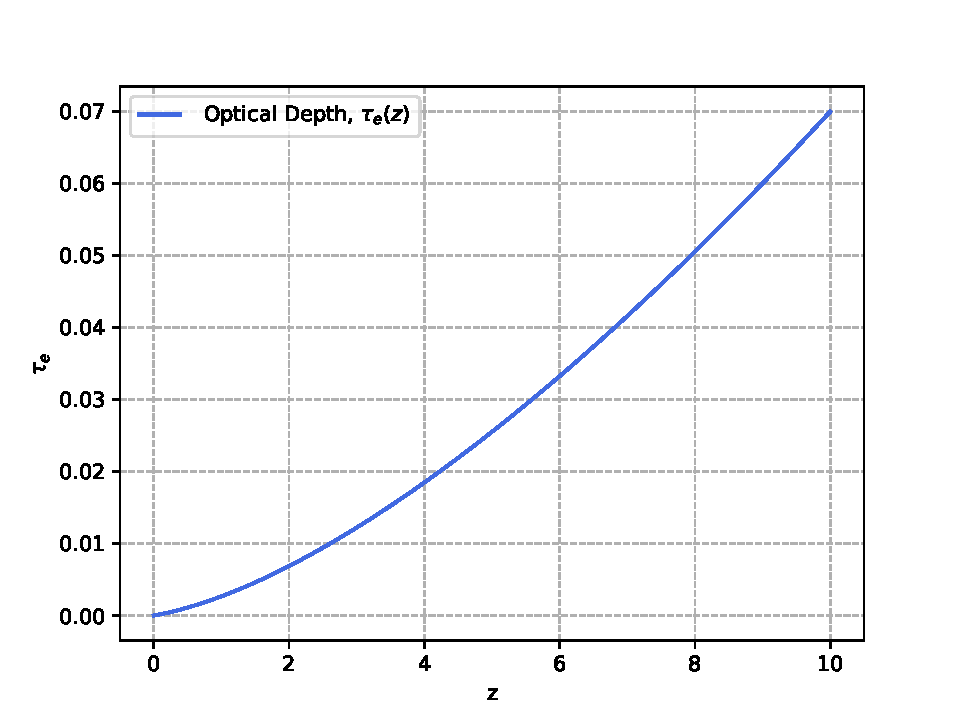
\includegraphics[width = \textwidth]{tau.pdf}
    \caption{The optical depth $\tau_e(z)$ of the IGM for redshift $z\in [0,10]$.}
    \label{fig:tau}
\end{figure}

\section*{Exercise 3}
\subsection*{a)}

In the lectures we derived the following second order differential equation for the
density profile of an "isothermal" halo

\begin{equation}\label{eq:halo}
    -\frac{k_b T}{m_{\text{DM}}r^2} \frac{d}{dr} r^2 \frac{d}{dr} \ln{\rho(r)} = 4\pi G
    \rho(r).
\end{equation}

\noindent We can show that

\begin{equation}\label{eq:halodef}
    \rho(r) = \frac{A}{r^2}, \qquad A = \frac{k_bT}{2\pi G m_{\text{DM}}},
\end{equation}
is a solution to equation \eqref{eq:halo} by substituting it in to the LHS.
We start by rewriting the logarithm expression to the form

\begin{equation*}
    \frac{d \ln(\rho)}{dr} = \frac{1}{\rho} \frac{d \rho}{dr}.
\end{equation*}

\noindent Next up, we insert for $\rho$ and compute the derivative

\begin{equation*}
    \frac{1}{\rho} \frac{d \rho}{dr} = \frac{r^2}{A} \frac{d}{dr} \left( \frac{A}{r^2}
    \right) = -\frac{2}{r}. 
\end{equation*}

\noindent Inserting this into equation \eqref{eq:halo} and computing the remaining
derivative
leaves us with

\begin{equation}\label{eq:halosub}
    \frac{2k_b T}{m_{\text{DM}}r^2} = 4\pi G \rho(r).
\end{equation}

\noindent If we now substitute the constants on the LHS with A, we find

\begin{equation*}
    \frac{k_b T}{m_\text{DM}} = 2\pi G A.
\end{equation*}

\noindent Finally we insert this into \eqref{eq:halosub}

\begin{equation*}
    4\pi G \frac{A}{r^2} = 4\pi G \rho(r).
\end{equation*}

\noindent By reinserting for $\rho(r)$ from definition \eqref{eq:halodef}, we see that
this is
indeed the solution.

\subsubsection*{b)}

For an isothermal gas, we have the following equation of state

\begin{equation}\label{eq:isoEOS}
    p = \frac{k_b T}{m_\text{p}} \rho.
\end{equation}

\noindent For a gas in hydrostatic equilibrium we have

\begin{equation}\label{eq:hydrostatic}
    \frac{dp}{dr} = - \frac{GM(<r)\rho}{r^2}.
\end{equation}

\noindent We will now show that an isothermal gas will end up in a similar state. We
assume
that the density profile is given similar to that of the isothermal halo, so that 

\begin{equation*}
    \rho (r) = \frac{A_\text{gas}}{r^2}, \qquad  A_\text{gas}  = \frac{k_b T}{2\pi G
    m_\text{p}}.
\end{equation*}

\noindent Rewriting the pressure in equation \eqref{eq:isoEOS} in terms of $ A_\text{gas} $
results in

\begin{equation}\label{eq:eossub}
    p = 2\pi G  A_\text{gas}  \rho (r).
\end{equation}

\noindent For a spherical symmetric gas, the mass which is smaller than some radius $r$
is given as

\begin{equation}\label{eq:mass}
    M (<r) = 4\pi \int_0^r x^2 dx \rho(x)  = \frac{4\pi}{3}r^3\rho(r) .
\end{equation}

\noindent We can now rewrite equation \eqref{eq:eossub} in terms of $M $ from equation 
\eqref{eq:mass}. Doing so leaves us with the following equation of state

\begin{equation}\label{eq:eossub2}
    p = \frac{3}{2} \frac{G M (<r) \rho (r)}{r}.
\end{equation}

\noindent Finally, we differentiate equation \eqref{eq:eossub2} with respect to r which 
leaves us with 

\begin{equation}\label{eq:isohydro}
    \frac{dp}{dr} = \frac{-3GM(<r) \rho(r)}{r^2}.
\end{equation}

\noindent We see that this is a very similar to the non-isothermal case seen in equation
\eqref{eq:hydrostatic}, the only difference being the factor 3. In both scenarios, the
gas results in a state where

\begin{equation}\label{eq:hydroprop}
    \frac{dp}{dr} \propto \frac{M(<r)\rho(r)}{r^2}.
\end{equation}

\end{document}